%% implementation

\section{SPHLATCH - An implementation}

This section shows an approach to parallelize a Barnes \& Hut tree in an easy way. A few code examples are given in C/C++.

\subsection{Parallizing a particle calculation}
To speed up a particle calculation, it is desirable to be able to let it run in parallel on multiple processors. There exist many different parallel setups, the one considered here consists of multiple processors with strictly local memory not directly accessible by the remote processors. Interprocessor communication is possible through an API like MPI.\\

The computational cost for calculating the derivatives like acceleration due to gravity or some SPH-sum in an SPH calculation, is typically of the same magnitude for every single particle. So a natural way of parallelizing such a calculation is to divide the set of particles used in the calculation into about equally sized subsets. Each subset is then assigned to a process on a processor. These subsets can be created by subdividing the space in which all particles lie into computational domains, an volume containing the desired subset of particles. For the parallelization method used for the tree, it is necessary to build these volumes using cubes with a side length of $\frac{l}{2^{n}}$, where $l$ is the side length of the root node of the octree.

\begin{figure}[htbp]
\begin{center}
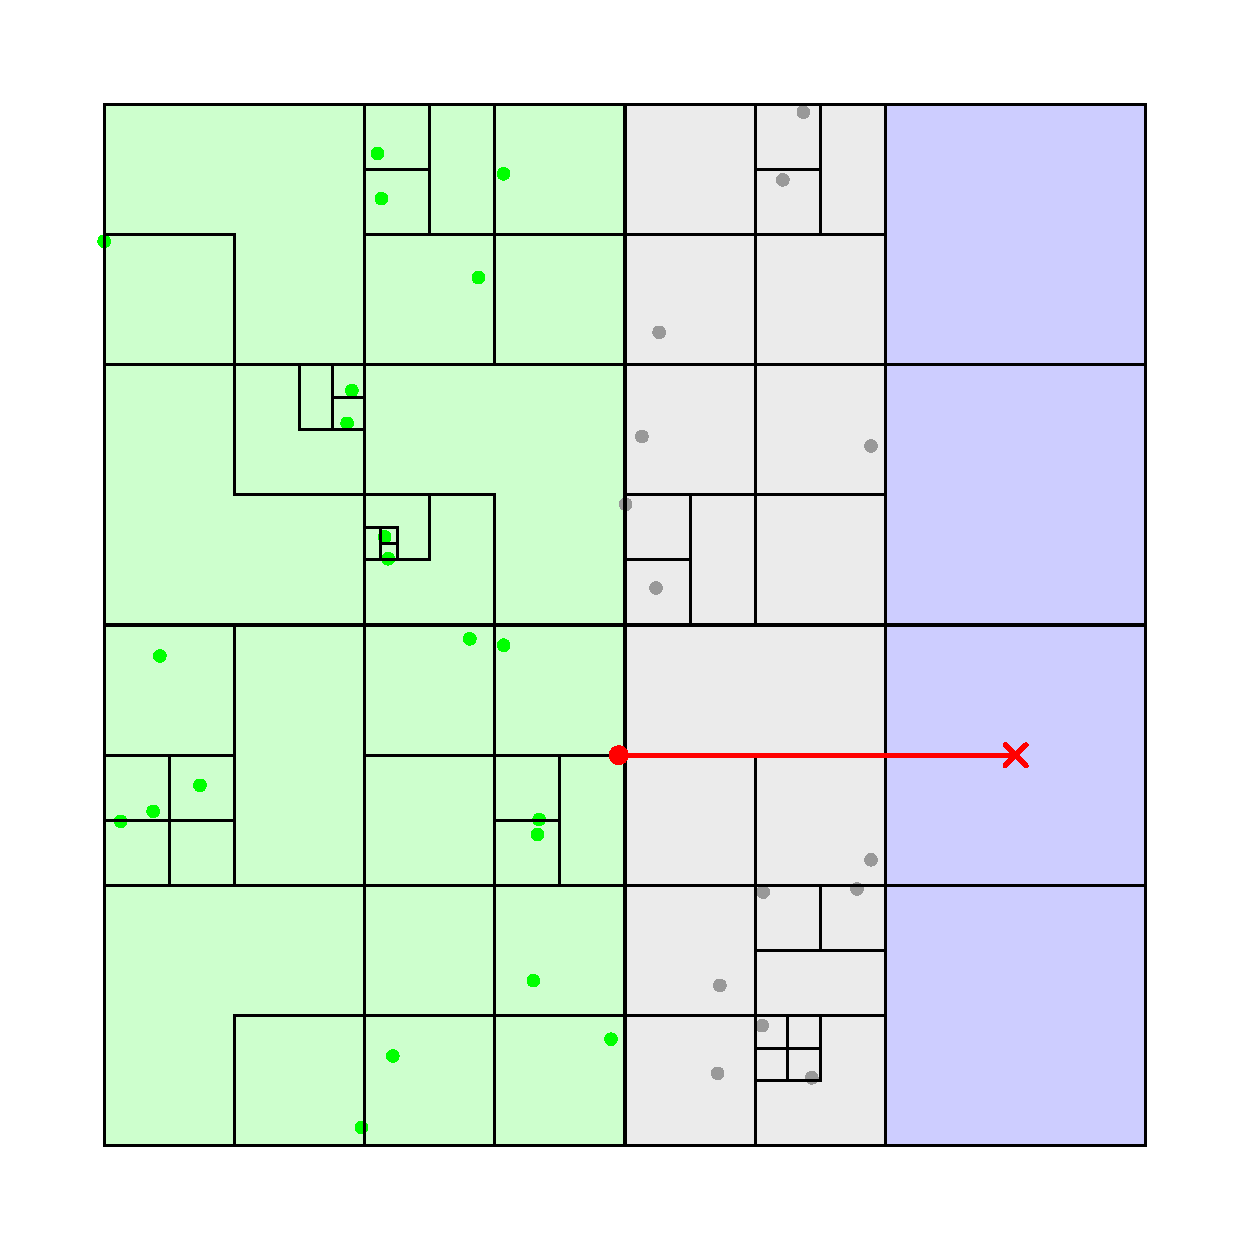
\includegraphics[scale=0.6]{quadtree50_xy_TPL2.pdf}
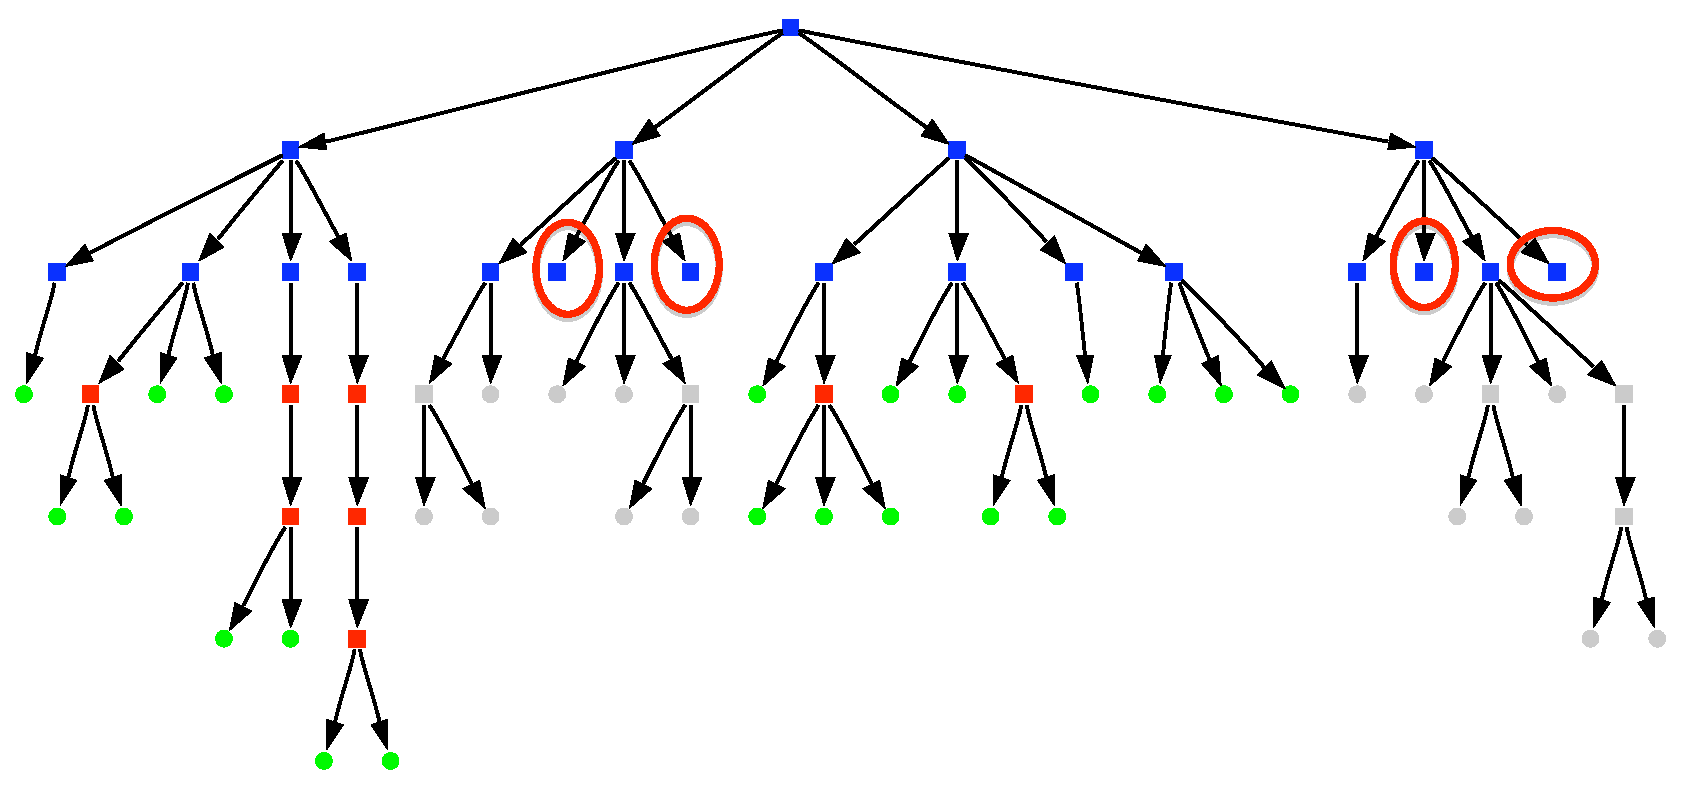
\includegraphics[scale=0.3]{quadtree50_TPL2.pdf}
\caption{the same 50 particles randomly distributed in $2D$}
\caption{A part of the same particle distribution like in figure \ref{fig:2D_BHtree}. The local domain is shaded green and contains 21 particles for which the acceleration has to be calculated. Bordering this zone is the ghost domain shaded grey, for which all particles are known. Beyond that, no particle information is available, only the corresponding parts of the global tree down to top-tree depth are known here. The plot below shows the corresponding tree. Note the filled top-tree nodes without any children nodes, they correspond to the domain where no particle information is available.}
\label{fig:2D_BHtree_costzone}
\end{center}
\end{figure}



costzone stuff

\subsection{Parallizing a B\&H-tree}
node specialization: toptree node, local vs. non-local nodes and particles
toptree recursion
costzone vs. toptree business
advantage: bulk communication
disadvantage: high memory usage

\subsection{Implementing a tree datastructure}
The most common and probably also easiest way to implement a tree datastructure is by using \emph{pointers}. Pointers are a datatype pointing to another datatype, which can be a pointer again. One now defines a node datastructure, which is made up of pointers to others nodes, namely the parent node and the children node. If a child does not exist, corresponding pointer is set to the null pointer. As there may be more than one child, an array is used to store the child pointers with a size corresponding to the maximum number of children. Other information can also be stored in the tree node, for example in the case of a Barnes \& Hut tree the depth and the center coordinates of a cell.
\begin{verbatim}
struct node {
    node* parent;
    node* child[8];    // an octree
    int depth;
    
    // let's store some useful data on this node
    float centerX, centerY, centerZ;
    ...
}
\end{verbatim}

The tree can now be contructed by letting the nodes point to each other. If we don't want to have to access the tree nodes explicitely, it is necessary to define a \emph{cursor}. The cursor is a node pointer and can therefore point to any node in the tree. Data of the nodes can be accessed through the cursor. 
\begin{verbatim}
...
// assume we have the tree: Root -> Child0 -> Grandchild3
node* Cursor;
Cursor = *Root;               // initialize the Cursor
Cursor = Cursor->child[0];    // Cursor now points to Child0
Cursor->centerX = 42.;        // set centerX of Childo to 42
Cursor = Cursor->child[3];    // Cursor now points to Grandchild3
Cursor = Cursor->parent;      // ... to Child0 again
...
\end{verbatim}

Elementary tree operations can now be implemented, like going up to the parent node or going to a child.\\

Tree walks can be implemented be implemented by recursive functions, so called \emph{recursors}:
\begin{verbatim}
void postorderRecursor() {
    // do something
    useful();
    
    // walk existing children
    for (size_t i = 0; i < 8; i++) {        // assume 8 childs
         if ( Cursor->child[i] != NULL ) {  // does the child exist?
             goChild(i);
             postorderRecursor();           // recurse
             goParent();
         }
    }
}
...
goRoot();               // go to the root node
postorderRecursor();    // walk the tree
...
\end{verbatim}

The cursor will point to every tree node once in a post order and every time the function \verb|useful()| is executed. A pre-order tree walk or a walk of a subtree can be implemented in a similar fashion.\\

Each time the recursor calls itself, the current context is laid on to the stack, so the stack-depth is incremented by one. On a real-world computer, the stack has a finite size. When we want to walk a tree with mind-blowing depth, the stack depth will increase the deeper we go in the tree and will possibly overflow, leading to a program crash. So is recursion dangerous for tree walks? In the case of Barnes \& Hut trees it is not.\\

This can be shown with a quick back of a napkin calculation: Let's imagine a worst-case scenario with two particles positioned at almost the same coordinates. When trying to insert the second particle at almost the same place like the first particle, the two come to lie in the same cell octant so that a new children cell has to be created at this octant. Each time this happens, the resolution to distinguish the two particles increase by two or in other words, the the difference in coordinates of the particles has to be half as small in order for the tree not to be able to distinguish the two particles again. Or we can also say, one more bit of the binary representation of the particles coordinates have to match each other. Particle coordinates are usually stored as floating point numbers. A floating point number is usually represented according to the \emph{IEEE 754} standard, with 24 bits precision for a single precision float and 53 bits for a double precision float. So in a worst case, the tree gets a depth of around 24 or 53, a depth which can be handled by the stacks of modern computers. And yet this worst-case is very pathological, as a calculation with such high dynamics easily leads to other problems like over- or underflows. Concluding we can say, that recursion for the B\&H-tree walks is not dangerous.

\subsection{Implementing a B\&H-tree}
The gravitational acceleration calculation with a parallelized B\&H-tree like shown before breaks down to 4 major steps: Building the top-tree, inserting the particles and ghosts, calculating the multipole moments and finally calculating the resulting acceleration on the particles. If the tree is not needed any more, the tree has also to be deleted. For this five steps, there exist easy recursive algorithms.\\

After the root node has been created, 

%top-tree build algorithm
\begin{algorithm}
\caption{top-tree build recursor}
\begin{algorithmic}
\label{alg:buildtoptree}
\IF{ depth $\ge$  top-tree depth}
\STATE{make emtpy cell node}
\FORALL{children}
\STATE{go to child}
\STATE{call top-tree build recursor}
\STATE{go to parent}
\ENDFOR
\ENDIF
\end{algorithmic}
\end{algorithm}

Inserting a particle into the tree can also be done with a recursive function. The idea is to start at the root node and try to insert the particle as a child of the current node. There are three cases possible: The child node does not exist, so the particle can be inserted directly. If there is already a cell node, go there and call the insertion function again. If there is already a particle node, save this particle temporarily and call the insertion function for this particle and the one that has been to be inserted in the first place. At the beginning of the recursor, the current node is set to be non-empty, so that the inserting a particle leaves a path from the root node to the particle of non-empty nodes.
%particle insertion algorithm
\begin{algorithm}
\caption{insert particle $p_{i}$ recursor}
\begin{algorithmic}
\label{alg:insertparticle}
\STATE{$k =$ subVolumeIndex($p_{i}$)}
\STATE{set current node to non-empty}
\IF{child $k$ is not existing }
\STATE{go to child $k$}
\STATE{make particle node, fill it with $p_{i}$}
\STATE{go to parent}
\ELSIF{child $k$ is a cell node}
\STATE{go to child $k$}
\STATE{call insert particle $p_{i}$ recursor}
\STATE{go to parent}
\ELSIF{child $k$ is a particle node}
\STATE{save particle from child $k$ to $p_{j}$}
\STATE{go to child $k$}
\STATE{convert particle node to cell node}
\STATE{call insert particle recursor for $p_{i}$}
\STATE{call insert particle recursor for $p_{j}$}
\STATE{go to parent}
\ENDIF
\end{algorithmic}
\end{algorithm}\\

When the tree has been built, the multipole moments can be calculated by iterating through all non-empty tree nodes in a pre-order fashion, so that the multipole moments of the children of a node are already calculated when the multipoles of the node has to be calculated. The multipoles calculation recursor starts at the root node. After its execution, all cell nodes below the top-tree contain the correct multipole moments, this is also the case for cell nodes containing only ghost nodes. After executing the recursor, the multipoles in the top-tree are added up globally, so that also the top-tree cell nodes contain the correct multipole moments. This is done by summing up between processes pair-wise with a binary tree, so that even for a high number of processes there are not too many communication steps. The total of the multipoles is then distributed again to every process with the same binary in the opposite direction.
%multipole calculation algorithm
\begin{algorithm}
\caption{multipoles calculation recursor}
\begin{algorithmic}
\label{alg:multipolecalc}
\IF{current node is not empty }
\FORALL{existing children}
\STATE{go to child}
\STATE{call multipoles calculation recursor}
\STATE{go to parent}
\IF{ depth $>$ top-tree depth }
\STATE{calculate multipoles from children nodes with the same locality}
\ELSE
\STATE{calculate multipoles from local children nodes}
\ENDIF
\ENDFOR
\ENDIF
\end{algorithmic}
\end{algorithm}
\\

To calculate the acceleration due to gravity for a particle, a recursive tree walk starting from the root node has to be undertaken. The recursion is stopped, when either the MAC is fulfilled or the current node is a particle or empty. In order not to calculate the gravitational interaction of the particle with itself, before calling the algorithm, the particle node is made to look like an empty cell node, so that no interaction is calculated. After the execution of the algorithm, the corresponding node is changed back again to a particle node.
%acceleration algorithm
\begin{algorithm}
\caption{acceleration calculation recursor}
\begin{algorithmic}
\label{alg:calcgravity}
\IF{current node is a particle node}
\STATE{calculate acceleration due to a particle}
\ELSIF{current node is empty}
\STATE{do nothing}
\ELSIF{MAC is fulfilled}
\STATE{calculate acceleration due to a cell}
\ELSE
\FORALL{existing children}
\STATE{go to child}
\STATE{call acceleration calculation recursor}
\STATE{go to parent}
\ENDFOR
\ENDIF
\end{algorithmic}
\end{algorithm}\\

The tree has to be deleted again after the calculation. In order not to disconnect any nodes from the tree, the nodes are deleted in a pre-order fashion with algorithm \ref{alg:treedeletion}.
%tree deletion algorihm
\begin{algorithm}
\caption{tree deletion recursor}
\begin{algorithmic}
\label{alg:treedeletion}
\FORALL{children}
\STATE{go to child}
\STATE{call tree deletion recursor}
\STATE{go to parent}
\STATE{delete current node}
\ENDFOR
\end{algorithmic}
\end{algorithm}
